\documentclass[openany]{book}

%% Language and font encodings
\usepackage[english]{babel}
\usepackage[utf8x]{inputenc}
% \usepackage[T1]{fontenc}
\hyphenation{berke-ley}


%% Sets page size and margins
\usepackage[a4paper,top=2.5cm,bottom=2cm,left=3cm,right=3cm,marginparwidth=1.75cm]{geometry}

%% Useful packages
\usepackage{amsmath}
% \usepackage{graphicx}
\usepackage[colorlinks=true, allcolors=blue]{hyperref}
% \usepackage{apacite} % APA style citations
% \AtBeginDocument{\urlstyle{APACsame}}  % Links in APA citytions same formatting
% \usepackage{tabulary}
% \usepackage{natbib} % natbib citations: \citep{} and \citet{} for in-text
% \usepackage{booktabs}
\usepackage{pdfpages}
\usepackage{fancyhdr}
\pagestyle{fancy} % This must be here, because defaults are set and renewcommand for section marks will work.
\fancyhf{} % sets both header and footer to nothing
\renewcommand{\headrulewidth}{0pt} % No rhead rule
% \fancyfoot[C]{\thepage} % Centered page number
%\fancyhead[L]{\small \leftmark} % Chapter title on the left
%\fancyhead[R]{Page\thepage} % Chapter title on the left
% Redefine chapter mark to include section number
% \renewcommand{\chaptermark}[1]{\markboth{CHAPTER \thechapter.\thesection\ #1}{}}
% \renewcommand{\sectionmark}[1]{\markright{}}
% \setlength{\headheight}{5pt} % Adjust as needed
% \setlength{\headsep}{20pt}    % Increase space between header and text
% Remove underlining from headers
% \renewcommand{\chaptermark}[1]{\markboth{\thechapter\ #1}{}}
\usepackage{todonotes}
\usepackage{tocloft}
% Increase spacing between entries
\setlength{\cftbeforechapskip}{3em} % Adjust chapter spacing
\setlength{\cftbeforesecskip}{1.5em}    % Adjust section spacing
% Increase font size
\renewcommand{\cftchapfont}{\large\bfseries} % Chapter titles
\renewcommand{\cftsecfont}{\large}           % Section titles
% Remove indent for line-broken subsections
% \setlength{\cftsecindent}{0pt}
% If you use \tableofcontents, this adjusts the name
\addto\captionsenglish{\renewcommand*\contentsname{Contents}}


\begin{document}

% \frontmatter
\pagenumbering{gobble}

%% \vspace{5cm}
%\begin{center}
%\hphantom{a} \\ \vspace{3cm}
%\begin{Large}
%\textbf{Africa's Economic Transformation: A Big Data\\Economic Perspective}
%\end{Large}
%
%\vspace{4cm}
%\begin{large}
%Inaugural-Dissertation \\
%zur Erlangung des akademischen Grades eines Doktors  \\
%der Wirtschafts- und Sozialwissenschaften \\
%der Wirtschafts- und Sozialwissenschaftlichen Fakultät \\
%der Christian-Albrechts-Universität zu Kiel \\
%\vspace{2cm}
%vorgelegt von \\
%MIE Sebastian Krantz \\
%aus Altenholz \\
%\vspace{2cm}
%Kiel, 21. August 2024
%\end{large}
%\end{center}

% Change footnote symbol to a star
\renewcommand{\thefootnote}{\fnsymbol{footnote}}

\begin{titlepage}
    \vspace*{\fill}
    \begin{center}
        \Huge\textbf{Africa's Economic Transformation}\\A Big Data Economic Perspective
        
        \vspace{1cm}
        \Large Sebastian Krantz\footnote{Kiel Institute for the World Economy\\ \textit{Address:} Haus Welt-Club, Duesternbrooker Weg 148, D-24105 Kiel\\ \textit{E-mail:} sebastian.krantz@ifw-kiel.de or sebastian.krantz@graduateinstitute.ch\\ \textit{Website:} \href{https://sebastiankrantz.com}{sebastiankrantz.com} and \href{https://www.ifw-kiel.de/experts/sebastian-krantz/}{ifw-kiel.de/experts/sebastian-krantz}}\\[1em]Inaugural Dissertation for a PhD in Quantitative Economics\\by the University of Kiel, in Partnership with the\\Kiel Institute for the World Economy
\\[1em]August 21, 2024
        
        
        \vspace{2cm} % 2cm
        \large \textbf{Abstract}
        
        \vspace{0.5cm}
        \begin{minipage}{0.9\textwidth}
            \normalsize
            \hphantom{aa.}Africa is a continent of great economic potential. With a population of 1.5 billion at a median age of 19 today, projected to reach 2.5 billion by 2050, vast natural and mineral resources, yet a share of only $\sim$3\% in global GDP and trade, Africa's economic transformation must materialize to provide opportunities for its youth and to foster a more balanced, equitable, and secure world order in the face of shared global challenges. The African Union's Agenda 2063 sets an ambitious path to achieve this, and with the formal enactment of a continental free trade area, a substantial landmark has been passed. However, trade and regional value chains (RVCs) must pick up significantly to generate the desired economic transformation, supported by industrialization and increases in productivity. For this, macroeconomic and financial stability are needed alongside industrial/RVC policies and large-scale investments in infrastructure and human capital. This doctoral dissertation contributes to our understanding of these critical ingredients. It documents the continent's progress in macroeconomic stability and investigates its drivers. It also dissects Africa's integration into global and regional value chains, eliciting progress, benefits, potentials, and challenges towards/of regional economic integration. Last but not least, it zooms in on the continent's infrastructure, utilizing geospatial big data and modern structural and empirical methods to provide evidence on local and global investment potentials at unprecedented spatial detail and scale. By combining rigorous quantitative economics and (causal) machine learning with the richest data on global production, trade, infrastructure, and economic geography available at the time of writing, it produces very detailed and substantive evidence on critical aspects of Africa's present and future economic transformation. It thus enhances our academic understanding of the continent, its economic potential and challenges, but also informs policies to accelerate economic progress and transformation at scale. \\\\\\
\noindent \textbf{Keywords:} Africa, economic transformation and development, infrastructure,\\\hphantom{a a a a a a a.}roads, spatially optimal investments, regional integration, trade, GVCs,\\\hphantom{a a a a a a a.}RVCs, EAC, macoeconomic stability, growth, volatility, structural change,\\\hphantom{a a a a a a a.}big data, partial and general equilibrium, causal ML, XAI\\\\
\textbf{JEL Classification:} F14; F15; O11; O18; R42; R10; O10; O11; E30; E60
        \end{minipage}
    \end{center}
    \vspace*{\fill}
\end{titlepage}

%% Empty page
%% \newpage
\hphantom{a}
\newpage

% Revert back to numbered footnotes
\renewcommand{\thefootnote}{\arabic{footnote}}
\setcounter{footnote}{0}

% \mainmatter


%----------------------------------------------------------------------------------
% Content
%----------------------------------------------------------------------------------

\tableofcontents
\newpage

\pagenumbering{arabic}
\chapter{Introduction}
\thispagestyle{empty} 
% \addtocounter{page}{-1} % Adjust the page counter
\newpage

% Need to place here to not have "Page" on the title page
\fancyhead[L]{\small \leftmark} % Chapter title on the left
\fancyhead[R]{Page \thepage} % Chapter title on the left
\markboth{CHAPTER 1. INTRODUCTION}{}



% \section{Introduction}


\includepdf[page=-, pagecommand={\thispagestyle{fancy}}, fitpaper=true]{"introduction.pdf"}

\chapter{Macroeconomic Stabilization}
\thispagestyle{empty}
% \addtocounter{page}{-1} % Adjust the page counter
\newpage


% Add section to TOC without displaying it
\phantomsection
\addcontentsline{toc}{section}{2.1\ \ Africa's Great Moderation}
% \section{Africa's Great Moderation}
\markboth{CHAPTER 2.1. AFRICA'S GREAT MODERATION}{}

% \textbf{Submission Status:} Published, Journal of African Economies

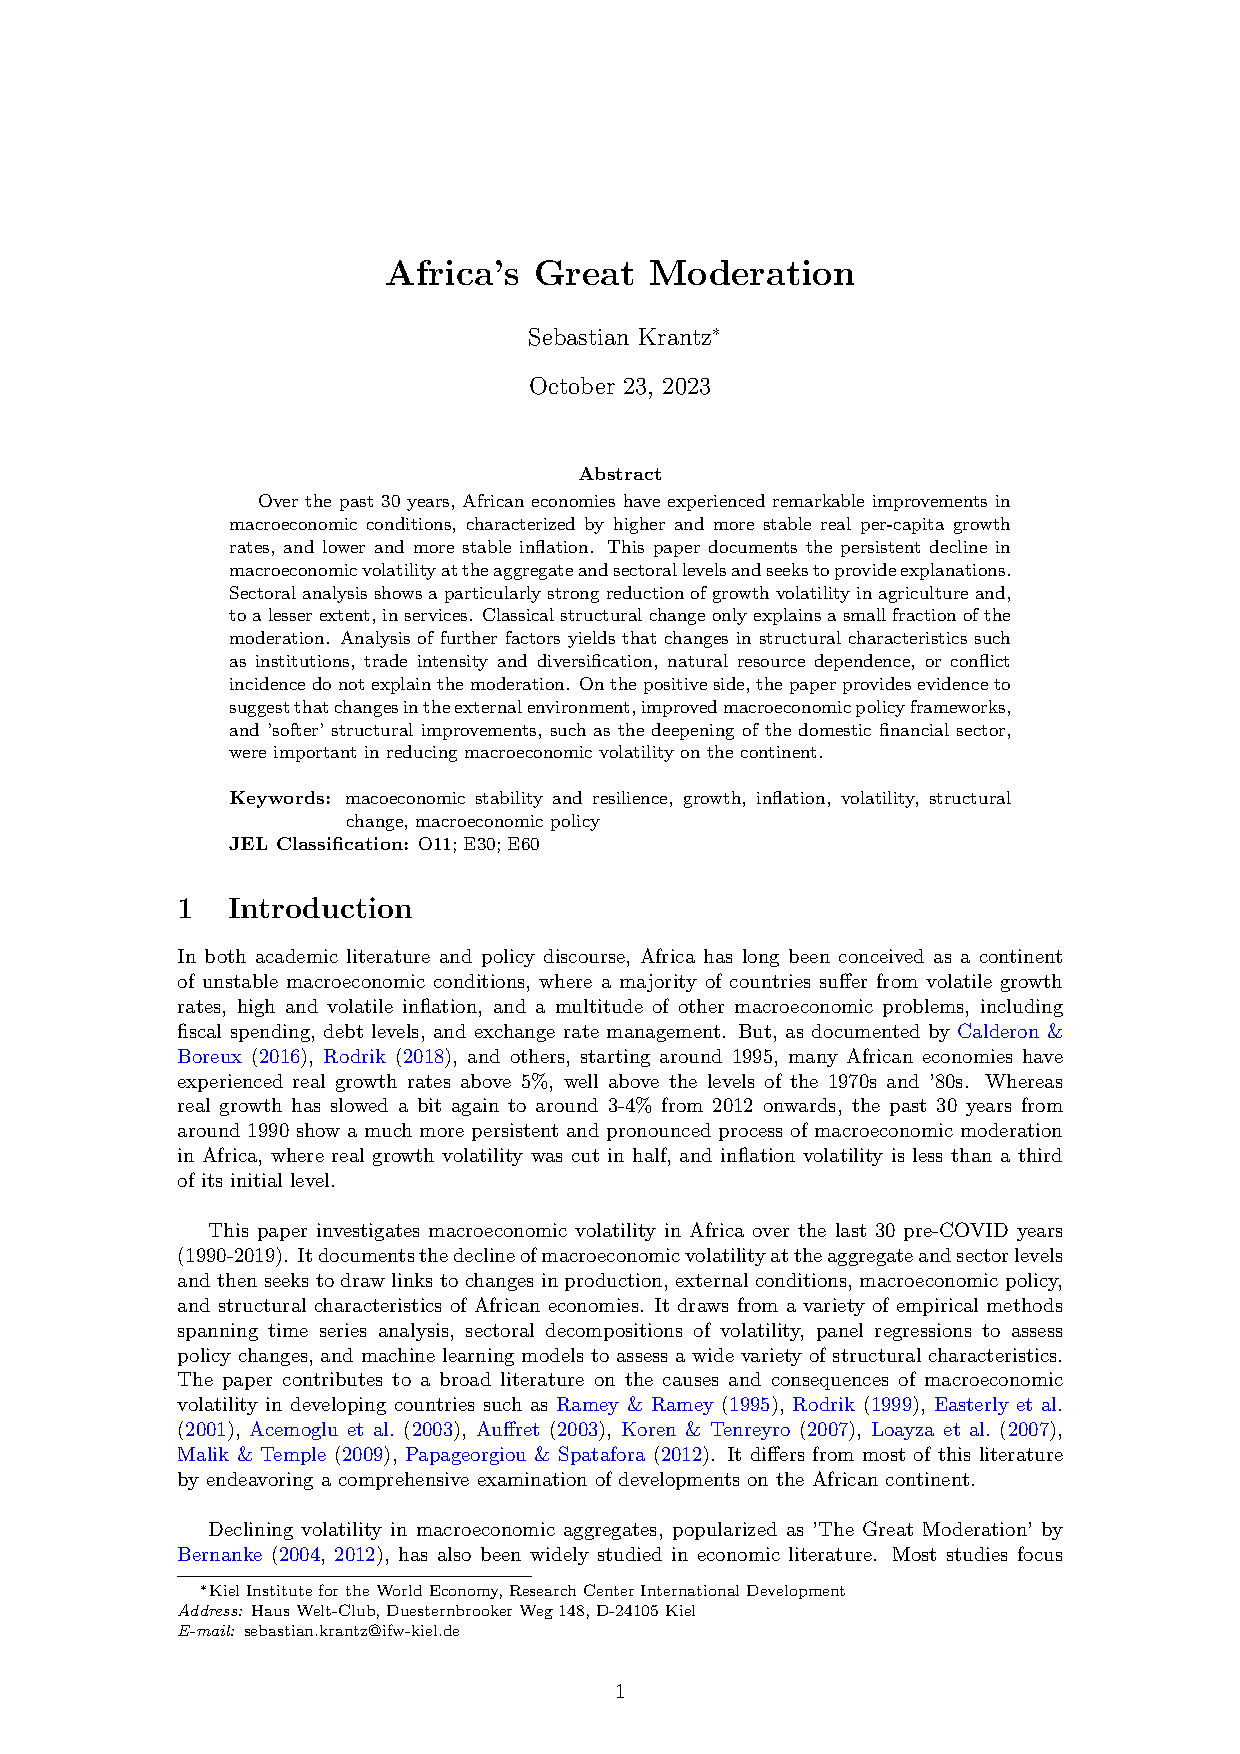
\includepdf[page=-, pagecommand={\thispagestyle{fancy}}, fitpaper=true]{"documents/africas_great_moderation.pdf"}

\chapter{Regional and Global Economic Integration}
\thispagestyle{empty}
% \addtocounter{page}{-1} % Adjust the page counter
\newpage

\phantomsection
\addcontentsline{toc}{section}{3.1\ \ Africa's Regional and Global Integration}
\markboth{CHAPTER 3.1. AFRICA'S REGIONAL AND GLOBAL INTEGRATION}{}

% \textbf{Submission Status:} This is some work for a background paper for the World Bank. I will include it in the dissertation because it provides the appropriate context for the EAC paper that follows.

\includepdf[page=-, pagecommand={\thispagestyle{fancy}}, fitpaper=true]{"documents/World Bank Africas Global and Regional Integration/main.pdf"} % 1-18

\phantomsection
\addcontentsline{toc}{section}{3.2\ \ Patterns of Global and Regional Integration in the East\\African Community}
\markboth{CHAPTER 3.2. GLOBAL AND REGIONAL INTEGRATION IN THE EAC}{}

% \textbf{Submission Status:} Accepted, Review of World Economics, S.I. on Africa's Global and Regional Integration

\includepdf[page=-, pagecommand={\thispagestyle{fancy}}, fitpaper=true]{"documents/PoGaRIitEAC_Krantz.pdf"} % 1-37

\chapter{Infrastructure for Trade and Structural Transformation}
\thispagestyle{empty}
% \addtocounter{page}{-1} % Adjust the page counter
\newpage

\phantomsection
\addcontentsline{toc}{section}{4.1\ \ Mapping Africa's Infrastructure Potential with Geospatial\\Big Data and Causal ML}
\markboth{CHAPTER 4.1. MAPPING AFRICA'S INFRASTRUCTURE POTENTIAL}{}
% \textbf{Submission Status:} SSRN Working Paper

\includepdf[page=-, pagecommand={\thispagestyle{fancy}}, fitpaper=true]{"documents/mapping_africas_infrastructure_potential_Krantz0824.pdf"} % 1-32

\phantomsection
\addcontentsline{toc}{section}{4.2\ \ Optimal Investments in Africa's Road Network}
\markboth{CHAPTER 4.2. OPTIMAL INVESTMENTS IN AFRICA'S ROAD NETWORK}{}

% \textbf{Submission Status:} Kiel Working Paper and World Bank Policy Research Working Paper (under Review at the Bank)

\includepdf[page=-, pagecommand={\thispagestyle{fancy}}, fitpaper=true]{"documents/optimal_investments_in_africas_road_network_Krantz0724.pdf"} % 1-58

% \section{Conclusion}


%----------------------------------------------------------------------------------
% Appendix
%----------------------------------------------------------------------------------
\appendix

\chapter{Acknowledgements}
\thispagestyle{empty}
\newpage

\hphantom{a}
\vspace{1cm}

I extend my greatest appreciation and gratitude to my supervisors, Prof. Tobias Heidland, Prof. Rainer Thiele, and Prof. Christoph Trebesch, for their invaluable input and support on the different papers of this dissertation and other research and organizational matters. In particular, Prof. Heidland has been enormously helpful in holding regular meetings to discuss my research, reading my drafts and providing useful comments, guiding me through publication processes, supporting research and conference visits abroad, and ensuring a rapid progression toward the PhD defense. I also thank Prof. Thiele for organizing conferences and activities within the Africa Initiative and providing valuable networking platforms and opportunities to present my research. In particular, the IDOS conference 2022 in Bonn, which led to a special issue on Africa's Regional and Global Integration, and the MIASA Policy Conference 2023 in Accra, Ghana, where I could present my work on infrastructure, were exceptional experiences. Prof. Thiele has also helped guide me through the (substantial) revision needed to publish my EAC paper in the Review of World Economics. Prof. Trebesch has been helpful in his strong endorsement of my pursuit to investigate Africa's infrastructure with Big Data, its effects on economic activity, and investment potentials. It has been a fruitful endeavor that led to this dissertation's most substantive empirical works (Chapter 4). Prof. Trebesch also endorsed the Africa Monitor, helped with marketing it (alongside Prof. Heidland), and giving it a prominent place on the Kiel Institute website. \newline 

 I would also like to thank many other Kiel Institute colleagues who have inspired my research and provided valuable data and feedback. In particular, Hendrik Mahlkow, Sekou Metiki, Linda Maokomatanda, Julian Hinz, Frauke Steglich, Malte Becker, David Mihalyi, Sebastian Horn, Lukas Franz, Carsten Brockhaus, Alina Mulyukova and Prof. Jens-Boysen Hogrefe have assisted with feedback, data sharing, and inspirational thoughts and conversations. \newline
 
 Outside of the Kiel Institute I would like to thank Niclas Moneke (Oxford), Tillmann von Carnap (Stanford), Tilman Graff (Harvard), Giulio Schinaia (Chicago), Joshua Blumenstock (Berkeley), Woan Foong Wong (Oregon), Prof. Maximilian von Ehrlich (Bern), Joris Mueller (NUS) and anonymous referees for providing invaluable feedback and inspirational comments on my work. \newline 
 
 I would also like to thank seminar/conference participants in Berlin, Stuttgart, Dresden, Bonn, Stellenbosch, Milan, Kampala, Accra, Berkeley, Oxford, the World Bank, and Kiel for helpful questions and comments. \newline 
 
 Special thanks are due to Hylton Hollander (UCT), who invited me to Stellenbosch and facilitated my research visit there, my lovely hosts Jurie and Magdaleen Goosen during this visit, Prof. Jens-Boysen Hogrefe for giving me the opportunity and supporting me in consulting GIZ and the Beninese Ministry of Finance on government revenue forecasting, Joshua Blumenstock (Berkeley) for inviting me to present my work at the Global Policy Lab, Diana Beltekian and Woubet Kassa (World Bank) for inviting me to participate in a World Bank report on Africa's regional integration which I continue to enjoy, Prof. Stefan Kooths for providing vital inputs on the user interface of the Africa Monitor, the Kiel Institute IT department, in particular Christoph Schweickhardt, for procuring the server and facilitating the launch of the Africa Monitor and its later transition into the hands of Eisenschmidt Consulting, several Kiel Institute researchers for contributing data stories to the Africa Monitor, and Daan Steenkamp and Byron Botha from Codera Analytics for hosting and maintaining the South Africa Macroeconomic Database and the SA Nowcasting platform that I built accompanying my research visit. \newline 
 
 Last but not least, I would like to thank my family and friends, particularly my parents and my lovely flatmates Sekou Metiki and Linda Maokomatanda, for providing social and emotional support during this, in many ways lonely and exhausting, journey of doctoral studies. % towards obtaining a PhD. 

% \section{Appendices}

%\subsection*{Africa's Great Moderation}
%
%\includepdf[page=-]{"documents/africas_great_moderation_22-end.pdf"}
%
%\subsection*{Africa's Regional and Global Integration}
%
%\includepdf[page=19-]{"documents/World Bank Africas Global and Regional Integration/main.pdf"}
%
%\subsection*{Patterns of Global and Regional Integration in the East African Community}
%
%\includepdf[page=38-]{"documents/PoGaRIitEAC_Krantz.pdf"}
%
%\subsection*{Mapping Africa's Infrastructure Potential with Geospatial Big Data and Causal ML}
%
%\includepdf[page=33-]{"documents/mapping_africas_infrastructure_potential_Krantz0824.pdf"}
%
%\subsection*{Optimal Investments in Africa's Road Network}
%
%\includepdf[page=59-]{"documents/optimal_investments_in_africas_road_network_Krantz0724.pdf"}


\newpage
\chapter[Declarations]{Declarations}
\thispagestyle{empty}
\newpage
\hphantom{a}\\ \vspace{4cm}


{\fontfamily{lmss}\selectfont
{\LARGE\noindent\textbf{Declaration to confirm that the dissertation has been\\[0.3em]produced independently} }
} \\ \vspace{1cm}


\vspace{1cm}
\noindent 
I hereby declare that I have produced my doctoral thesis \glqq Africa's Economic Transformation: A Big Data Economic Perspective\grqq{} independently and without external assistance and that I have specifically marked all passages taken verbatim from other authors, as well as the statements in my work that are closely based on the ideas of other authors, and that I have cited the sources according to the guidelines given to me.

\vspace{2cm}
%\textbf{Date} \hspace{5cm} \textbf{Signature}

\begin{raggedright}
\begin{tabular}{@{}p{3.5in}@{}}
\hrulefill \\
Location, Date \hspace{2cm} Sebastian Krantz
\end{tabular}
\end{raggedright}




\end{document}